% Created by tikzDevice version 0.12.6 on 2026-09-22 18:57:13
% !TEX encoding = UTF-8 Unicode
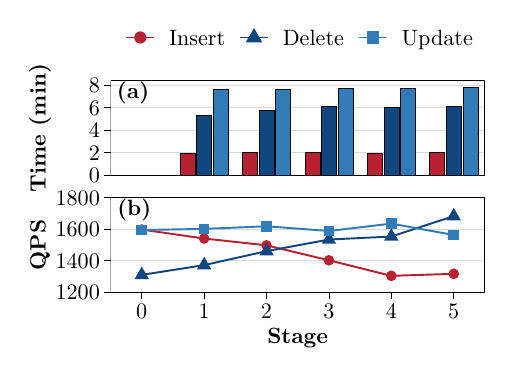
\begin{tikzpicture}[x=1pt,y=1pt]
\definecolor{fillColor}{RGB}{255,255,255}
\path[use as bounding box,fill=fillColor,fill opacity=0.00] (0,0) rectangle (166.22,115.63);
\begin{scope}
\path[clip] (  0.00,  0.00) rectangle (166.22,115.63);
\definecolor{drawColor}{RGB}{255,255,255}
\definecolor{fillColor}{RGB}{255,255,255}

\path[draw=drawColor,line width= 0.6pt,line join=round,line cap=round,fill=fillColor] (  0.00,  0.00) rectangle (166.22,115.63);
\end{scope}
\begin{scope}
\path[clip] (  0.00, 58.27) rectangle (166.22,115.63);
\definecolor{fillColor}{RGB}{255,255,255}

\path[fill=fillColor] (  0.00, 58.27) rectangle (166.22,115.63);
\end{scope}
\begin{scope}
\path[clip] (  0.00,  0.00) rectangle (166.22, 58.27);
\definecolor{fillColor}{RGB}{255,255,255}

\path[fill=fillColor] (  0.00,  0.00) rectangle (166.22, 58.27);
\end{scope}
\begin{scope}
\path[clip] ( 29.95, 62.27) rectangle (165.22, 96.52);
\definecolor{fillColor}{RGB}{255,255,255}

\path[fill=fillColor] ( 29.95, 62.27) rectangle (165.22, 96.52);
\definecolor{drawColor}{gray}{0.85}

\path[draw=drawColor,line width= 0.3pt,line join=round] ( 29.95, 62.27) --
	(165.22, 62.27);

\path[draw=drawColor,line width= 0.3pt,line join=round] ( 29.95, 70.42) --
	(165.22, 70.42);

\path[draw=drawColor,line width= 0.3pt,line join=round] ( 29.95, 78.58) --
	(165.22, 78.58);

\path[draw=drawColor,line width= 0.3pt,line join=round] ( 29.95, 86.73) --
	(165.22, 86.73);

\path[draw=drawColor,line width= 0.3pt,line join=round] ( 29.95, 94.89) --
	(165.22, 94.89);
\definecolor{fillColor}{RGB}{183,34,48}

\path[fill=fillColor] ( 55.05, 62.27) rectangle ( 60.46, 70.37);

\path[fill=fillColor] ( 77.59, 62.27) rectangle ( 83.01, 70.48);

\path[fill=fillColor] (100.14, 62.27) rectangle (105.55, 70.65);

\path[fill=fillColor] (122.69, 62.27) rectangle (128.10, 70.40);

\path[fill=fillColor] (145.23, 62.27) rectangle (150.64, 70.48);
\definecolor{fillColor}{RGB}{16,70,128}

\path[fill=fillColor] ( 61.06, 62.27) rectangle ( 66.47, 84.09);

\path[fill=fillColor] ( 83.61, 62.27) rectangle ( 89.02, 85.78);

\path[fill=fillColor] (106.15, 62.27) rectangle (111.56, 87.08);

\path[fill=fillColor] (128.70, 62.27) rectangle (134.11, 86.73);

\path[fill=fillColor] (151.24, 62.27) rectangle (156.65, 87.26);
\definecolor{fillColor}{RGB}{49,124,183}

\path[fill=fillColor] ( 67.07, 62.27) rectangle ( 72.48, 93.44);

\path[fill=fillColor] ( 89.62, 62.27) rectangle ( 95.03, 93.53);

\path[fill=fillColor] (112.16, 62.27) rectangle (117.57, 93.71);

\path[fill=fillColor] (134.71, 62.27) rectangle (140.12, 93.80);

\path[fill=fillColor] (157.25, 62.27) rectangle (162.67, 93.92);
\definecolor{drawColor}{RGB}{0,0,0}

\path[draw=drawColor,line width= 0.2pt] ( 55.05, 62.27) rectangle ( 60.46, 70.37);

\path[draw=drawColor,line width= 0.2pt] ( 77.59, 62.27) rectangle ( 83.01, 70.48);

\path[draw=drawColor,line width= 0.2pt] (100.14, 62.27) rectangle (105.55, 70.65);

\path[draw=drawColor,line width= 0.2pt] (122.69, 62.27) rectangle (128.10, 70.40);

\path[draw=drawColor,line width= 0.2pt] (145.23, 62.27) rectangle (150.64, 70.48);

\path[draw=drawColor,line width= 0.2pt] ( 61.06, 62.27) rectangle ( 66.47, 84.09);

\path[draw=drawColor,line width= 0.2pt] ( 83.61, 62.27) rectangle ( 89.02, 85.78);

\path[draw=drawColor,line width= 0.2pt] (106.15, 62.27) rectangle (111.56, 87.08);

\path[draw=drawColor,line width= 0.2pt] (128.70, 62.27) rectangle (134.11, 86.73);

\path[draw=drawColor,line width= 0.2pt] (151.24, 62.27) rectangle (156.65, 87.26);

\path[draw=drawColor,line width= 0.2pt] ( 67.07, 62.27) rectangle ( 72.48, 93.44);

\path[draw=drawColor,line width= 0.2pt] ( 89.62, 62.27) rectangle ( 95.03, 93.53);

\path[draw=drawColor,line width= 0.2pt] (112.16, 62.27) rectangle (117.57, 93.71);

\path[draw=drawColor,line width= 0.2pt] (134.71, 62.27) rectangle (140.12, 93.80);

\path[draw=drawColor,line width= 0.2pt] (157.25, 62.27) rectangle (162.67, 93.92);

\node[text=drawColor,anchor=base west,inner sep=0pt, outer sep=0pt, scale=  0.80] at ( 32.27, 89.89) {\bfseries (a)};

\path[draw=drawColor,line width= 0.4pt,line join=round,line cap=round] ( 29.95, 62.27) rectangle (165.22, 96.52);
\end{scope}
\begin{scope}
\path[clip] (  0.00,  0.00) rectangle (166.22,115.63);
\definecolor{drawColor}{RGB}{0,0,0}

\node[text=drawColor,anchor=base east,inner sep=0pt, outer sep=0pt, scale=  0.80] at ( 26.07, 59.51) {0};

\node[text=drawColor,anchor=base east,inner sep=0pt, outer sep=0pt, scale=  0.80] at ( 26.07, 67.67) {2};

\node[text=drawColor,anchor=base east,inner sep=0pt, outer sep=0pt, scale=  0.80] at ( 26.07, 75.82) {4};

\node[text=drawColor,anchor=base east,inner sep=0pt, outer sep=0pt, scale=  0.80] at ( 26.07, 83.98) {6};

\node[text=drawColor,anchor=base east,inner sep=0pt, outer sep=0pt, scale=  0.80] at ( 26.07, 92.13) {8};
\end{scope}
\begin{scope}
\path[clip] (  0.00,  0.00) rectangle (166.22,115.63);
\definecolor{drawColor}{RGB}{0,0,0}

\path[draw=drawColor,line width= 0.3pt,line join=round] ( 27.67, 62.27) --
	( 29.95, 62.27);

\path[draw=drawColor,line width= 0.3pt,line join=round] ( 27.67, 70.42) --
	( 29.95, 70.42);

\path[draw=drawColor,line width= 0.3pt,line join=round] ( 27.67, 78.58) --
	( 29.95, 78.58);

\path[draw=drawColor,line width= 0.3pt,line join=round] ( 27.67, 86.73) --
	( 29.95, 86.73);

\path[draw=drawColor,line width= 0.3pt,line join=round] ( 27.67, 94.89) --
	( 29.95, 94.89);
\end{scope}
\begin{scope}
\path[clip] (  0.00,  0.00) rectangle (166.22,115.63);
\definecolor{drawColor}{RGB}{0,0,0}

\node[text=drawColor,rotate= 90.00,anchor=base,inner sep=0pt, outer sep=0pt, scale=  0.80] at (  6.52, 79.39) {\bfseries Time (min)};
\end{scope}
\begin{scope}
\path[clip] ( 29.95, 20.02) rectangle (165.22, 54.27);
\definecolor{fillColor}{RGB}{255,255,255}

\path[fill=fillColor] ( 29.95, 20.02) rectangle (165.22, 54.27);
\definecolor{drawColor}{gray}{0.85}

\path[draw=drawColor,line width= 0.3pt,line join=round] ( 29.95, 20.02) --
	(165.22, 20.02);

\path[draw=drawColor,line width= 0.3pt,line join=round] ( 29.95, 31.43) --
	(165.22, 31.43);

\path[draw=drawColor,line width= 0.3pt,line join=round] ( 29.95, 42.85) --
	(165.22, 42.85);

\path[draw=drawColor,line width= 0.3pt,line join=round] ( 29.95, 54.27) --
	(165.22, 54.27);
\definecolor{drawColor}{RGB}{183,34,48}

\path[draw=drawColor,line width= 0.7pt,line join=round] ( 41.22, 42.67) --
	( 63.77, 39.44) --
	( 86.31, 36.98) --
	(108.86, 31.57) --
	(131.40, 25.96) --
	(153.95, 26.68);
\definecolor{drawColor}{RGB}{16,70,128}

\path[draw=drawColor,line width= 0.7pt,line join=round] ( 41.22, 26.30) --
	( 63.77, 29.83) --
	( 86.31, 34.88) --
	(108.86, 39.07) --
	(131.40, 40.16) --
	(153.95, 47.54);
\definecolor{drawColor}{RGB}{49,124,183}

\path[draw=drawColor,line width= 0.7pt,line join=round] ( 41.22, 42.51) --
	( 63.77, 42.92) --
	( 86.31, 43.86) --
	(108.86, 42.16) --
	(131.40, 44.83) --
	(153.95, 40.72);
\definecolor{fillColor}{RGB}{183,34,48}

\path[fill=fillColor] ( 41.22, 42.67) circle (  1.93);

\path[fill=fillColor] ( 63.77, 39.44) circle (  1.93);

\path[fill=fillColor] ( 86.31, 36.98) circle (  1.93);

\path[fill=fillColor] (108.86, 31.57) circle (  1.93);

\path[fill=fillColor] (131.40, 25.96) circle (  1.93);

\path[fill=fillColor] (153.95, 26.68) circle (  1.93);
\definecolor{fillColor}{RGB}{16,70,128}

\path[fill=fillColor] ( 41.22, 29.30) --
	( 43.82, 24.80) --
	( 38.62, 24.80) --
	cycle;

\path[fill=fillColor] ( 63.77, 32.83) --
	( 66.36, 28.33) --
	( 61.17, 28.33) --
	cycle;

\path[fill=fillColor] ( 86.31, 37.87) --
	( 88.91, 33.38) --
	( 83.72, 33.38) --
	cycle;

\path[fill=fillColor] (108.86, 42.06) --
	(111.45, 37.57) --
	(106.26, 37.57) --
	cycle;

\path[fill=fillColor] (131.40, 43.16) --
	(134.00, 38.66) --
	(128.81, 38.66) --
	cycle;

\path[fill=fillColor] (153.95, 50.53) --
	(156.54, 46.04) --
	(151.35, 46.04) --
	cycle;
\definecolor{fillColor}{RGB}{49,124,183}

\path[fill=fillColor] ( 39.29, 40.58) --
	( 43.15, 40.58) --
	( 43.15, 44.44) --
	( 39.29, 44.44) --
	cycle;

\path[fill=fillColor] ( 61.84, 41.00) --
	( 65.69, 41.00) --
	( 65.69, 44.85) --
	( 61.84, 44.85) --
	cycle;

\path[fill=fillColor] ( 84.38, 41.94) --
	( 88.24, 41.94) --
	( 88.24, 45.79) --
	( 84.38, 45.79) --
	cycle;

\path[fill=fillColor] (106.93, 40.23) --
	(110.79, 40.23) --
	(110.79, 44.09) --
	(106.93, 44.09) --
	cycle;

\path[fill=fillColor] (129.48, 42.91) --
	(133.33, 42.91) --
	(133.33, 46.76) --
	(129.48, 46.76) --
	cycle;

\path[fill=fillColor] (152.02, 38.79) --
	(155.88, 38.79) --
	(155.88, 42.65) --
	(152.02, 42.65) --
	cycle;
\definecolor{drawColor}{RGB}{0,0,0}

\node[text=drawColor,anchor=base west,inner sep=0pt, outer sep=0pt, scale=  0.80] at ( 32.40, 47.64) {\bfseries (b)};

\path[draw=drawColor,line width= 0.4pt,line join=round,line cap=round] ( 29.95, 20.02) rectangle (165.22, 54.27);
\end{scope}
\begin{scope}
\path[clip] (  0.00,  0.00) rectangle (166.22,115.63);
\definecolor{drawColor}{RGB}{0,0,0}

\node[text=drawColor,anchor=base east,inner sep=0pt, outer sep=0pt, scale=  0.80] at ( 26.07, 17.26) {1200};

\node[text=drawColor,anchor=base east,inner sep=0pt, outer sep=0pt, scale=  0.80] at ( 26.07, 28.68) {1400};

\node[text=drawColor,anchor=base east,inner sep=0pt, outer sep=0pt, scale=  0.80] at ( 26.07, 40.10) {1600};

\node[text=drawColor,anchor=base east,inner sep=0pt, outer sep=0pt, scale=  0.80] at ( 26.07, 51.51) {1800};
\end{scope}
\begin{scope}
\path[clip] (  0.00,  0.00) rectangle (166.22,115.63);
\definecolor{drawColor}{RGB}{0,0,0}

\path[draw=drawColor,line width= 0.3pt,line join=round] ( 27.67, 20.02) --
	( 29.95, 20.02);

\path[draw=drawColor,line width= 0.3pt,line join=round] ( 27.67, 31.43) --
	( 29.95, 31.43);

\path[draw=drawColor,line width= 0.3pt,line join=round] ( 27.67, 42.85) --
	( 29.95, 42.85);

\path[draw=drawColor,line width= 0.3pt,line join=round] ( 27.67, 54.27) --
	( 29.95, 54.27);
\end{scope}
\begin{scope}
\path[clip] (  0.00,  0.00) rectangle (166.22,115.63);
\definecolor{drawColor}{RGB}{0,0,0}

\path[draw=drawColor,line width= 0.3pt,line join=round] ( 41.22, 17.74) --
	( 41.22, 20.02);

\path[draw=drawColor,line width= 0.3pt,line join=round] ( 63.77, 17.74) --
	( 63.77, 20.02);

\path[draw=drawColor,line width= 0.3pt,line join=round] ( 86.31, 17.74) --
	( 86.31, 20.02);

\path[draw=drawColor,line width= 0.3pt,line join=round] (108.86, 17.74) --
	(108.86, 20.02);

\path[draw=drawColor,line width= 0.3pt,line join=round] (131.40, 17.74) --
	(131.40, 20.02);

\path[draw=drawColor,line width= 0.3pt,line join=round] (153.95, 17.74) --
	(153.95, 20.02);
\end{scope}
\begin{scope}
\path[clip] (  0.00,  0.00) rectangle (166.22,115.63);
\definecolor{drawColor}{RGB}{0,0,0}

\node[text=drawColor,anchor=base,inner sep=0pt, outer sep=0pt, scale=  0.80] at ( 41.22, 10.63) {0};

\node[text=drawColor,anchor=base,inner sep=0pt, outer sep=0pt, scale=  0.80] at ( 63.77, 10.63) {1};

\node[text=drawColor,anchor=base,inner sep=0pt, outer sep=0pt, scale=  0.80] at ( 86.31, 10.63) {2};

\node[text=drawColor,anchor=base,inner sep=0pt, outer sep=0pt, scale=  0.80] at (108.86, 10.63) {3};

\node[text=drawColor,anchor=base,inner sep=0pt, outer sep=0pt, scale=  0.80] at (131.40, 10.63) {4};

\node[text=drawColor,anchor=base,inner sep=0pt, outer sep=0pt, scale=  0.80] at (153.95, 10.63) {5};
\end{scope}
\begin{scope}
\path[clip] (  0.00,  0.00) rectangle (166.22,115.63);
\definecolor{drawColor}{RGB}{0,0,0}

\node[text=drawColor,anchor=base,inner sep=0pt, outer sep=0pt, scale=  0.80] at ( 97.58,  1.56) {\bfseries Stage};
\end{scope}
\begin{scope}
\path[clip] (  0.00,  0.00) rectangle (166.22,115.63);
\definecolor{drawColor}{RGB}{0,0,0}

\node[text=drawColor,rotate= 90.00,anchor=base,inner sep=0pt, outer sep=0pt, scale=  0.80] at (  6.52, 37.14) {\bfseries QPS};
\end{scope}
\begin{scope}
\path[clip] (  0.00,  0.00) rectangle (166.22,115.63);
\definecolor{fillColor}{RGB}{255,255,255}

\path[fill=fillColor] ( 34.30,107.52) rectangle (160.87,115.63);
\end{scope}
\begin{scope}
\path[clip] (  0.00,  0.00) rectangle (166.22,115.63);
\definecolor{drawColor}{RGB}{183,34,48}

\path[draw=drawColor,line width= 0.7pt,line join=round] ( 35.58,112.08) -- ( 45.82,112.08);
\definecolor{fillColor}{RGB}{183,34,48}

\path[fill=fillColor] ( 40.70,112.08) circle (  2.21);
\end{scope}
\begin{scope}
\path[clip] (  0.00,  0.00) rectangle (166.22,115.63);
\definecolor{drawColor}{RGB}{16,70,128}

\path[draw=drawColor,line width= 0.7pt,line join=round] ( 76.67,112.08) -- ( 86.91,112.08);
\definecolor{fillColor}{RGB}{16,70,128}

\path[fill=fillColor] ( 81.79,115.52) --
	( 84.77,110.36) --
	( 78.81,110.36) --
	cycle;
\end{scope}
\begin{scope}
\path[clip] (  0.00,  0.00) rectangle (166.22,115.63);
\definecolor{drawColor}{RGB}{49,124,183}

\path[draw=drawColor,line width= 0.7pt,line join=round] (119.58,112.08) -- (129.82,112.08);
\definecolor{fillColor}{RGB}{49,124,183}

\path[fill=fillColor] (122.49,109.86) --
	(126.91,109.86) --
	(126.91,114.29) --
	(122.49,114.29) --
	cycle;
\end{scope}
\begin{scope}
\path[clip] (  0.00,  0.00) rectangle (166.22,115.63);
\definecolor{drawColor}{RGB}{0,0,0}

\node[text=drawColor,anchor=base west,inner sep=0pt, outer sep=0pt, scale=  0.80] at ( 51.10,109.32) {Insert};
\end{scope}
\begin{scope}
\path[clip] (  0.00,  0.00) rectangle (166.22,115.63);
\definecolor{drawColor}{RGB}{0,0,0}

\node[text=drawColor,anchor=base west,inner sep=0pt, outer sep=0pt, scale=  0.80] at ( 92.19,109.32) {Delete};
\end{scope}
\begin{scope}
\path[clip] (  0.00,  0.00) rectangle (166.22,115.63);
\definecolor{drawColor}{RGB}{0,0,0}

\node[text=drawColor,anchor=base west,inner sep=0pt, outer sep=0pt, scale=  0.80] at (135.10,109.32) {Update};
\end{scope}
\end{tikzpicture}
